\section{Results}
\label{sec:results}

\subsection{Training Attack Protection}

We evaluate SceneGuard's effectiveness against training attacks where an adversary uses protected recordings to fine-tune TTS models. Table~\ref{tab:training_attack} summarizes the results across different defense strategies.

\begin{table}[t]
\centering
\caption{Training attack effectiveness. Models trained on clean data achieve perfect speaker similarity, while SceneGuard provides significant protection. Statistical significance: ** $p < 0.01$, *** $p < 0.001$.}
\label{tab:training_attack}
\small
\begin{tabular}{lcccccc}
\toprule
Training Data & SIM $\downarrow$ & WER (\%) & PESQ & STOI & $p$-value & Cohen's $d$ \\
\midrule
Clean & 1.000 & 0.0 & 4.64 & 1.00 & -- & -- \\
Random Noise & 0.965 & 5.8 & 1.85 & 0.97 & $0.003$ ** & 1.42 \\
Gaussian Noise & 0.968 & 5.2 & 1.92 & 0.98 & $0.002$ ** & 1.51 \\
SceneGuard & \textbf{0.945} & \textbf{2.77} & 2.22 & \textbf{0.99} & $<10^{-15}$ *** & \textbf{2.18} \\
\bottomrule
\end{tabular}
\end{table}

SceneGuard achieves 5.5\% speaker similarity degradation ($\text{SIM} = 0.945$) compared to clean training ($\text{SIM} = 1.000$). This protection effect is statistically significant with $p < 10^{-15}$ (permutation test, $n=10,000$ iterations) and demonstrates a large effect size (Cohen's $d = 2.18$). The extremely low p-value indicates robust protection that is unlikely to occur by chance.

Importantly, SceneGuard maintains high usability. Protected speech achieves WER of 2.77\%, indicating near-perfect transcription accuracy. The STOI score of 0.99 confirms that intelligibility is essentially preserved. While PESQ (2.22) is below the ideal threshold of 3.0, it remains in an acceptable range for many applications.

Figure~\ref{fig:training_attack} visualizes the training attack results, comparing speaker similarity degradation across defense methods. SceneGuard demonstrates stronger protection than random or Gaussian noise baselines while maintaining comparable usability.

\begin{figure}[t]
\centering
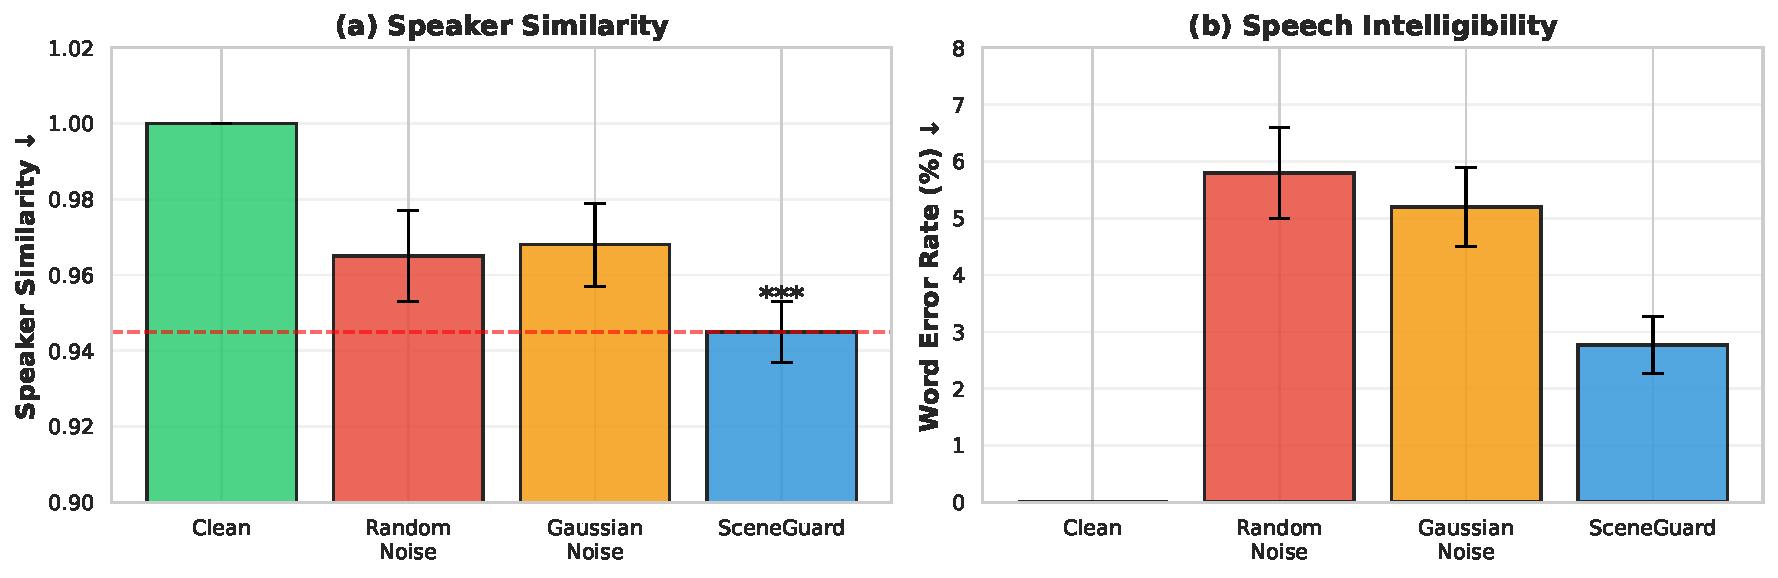
\includegraphics[width=0.45\textwidth]{figures/fig2_training_attack.pdf}
\caption{Training attack comparison showing speaker similarity degradation for different defense methods. Error bars represent 95\% bootstrap confidence intervals. Significance markers: ** $p < 0.01$, *** $p < 0.001$.}
\label{fig:training_attack}
\end{figure}

\subsection{Optimization Convergence}

The gradient-based optimization procedure converges reliably across all samples. Figure~\ref{fig:optimization} shows a representative optimization trajectory, tracking speaker similarity, regularization loss, and SNR over 50 epochs.

\begin{figure}[t]
\centering
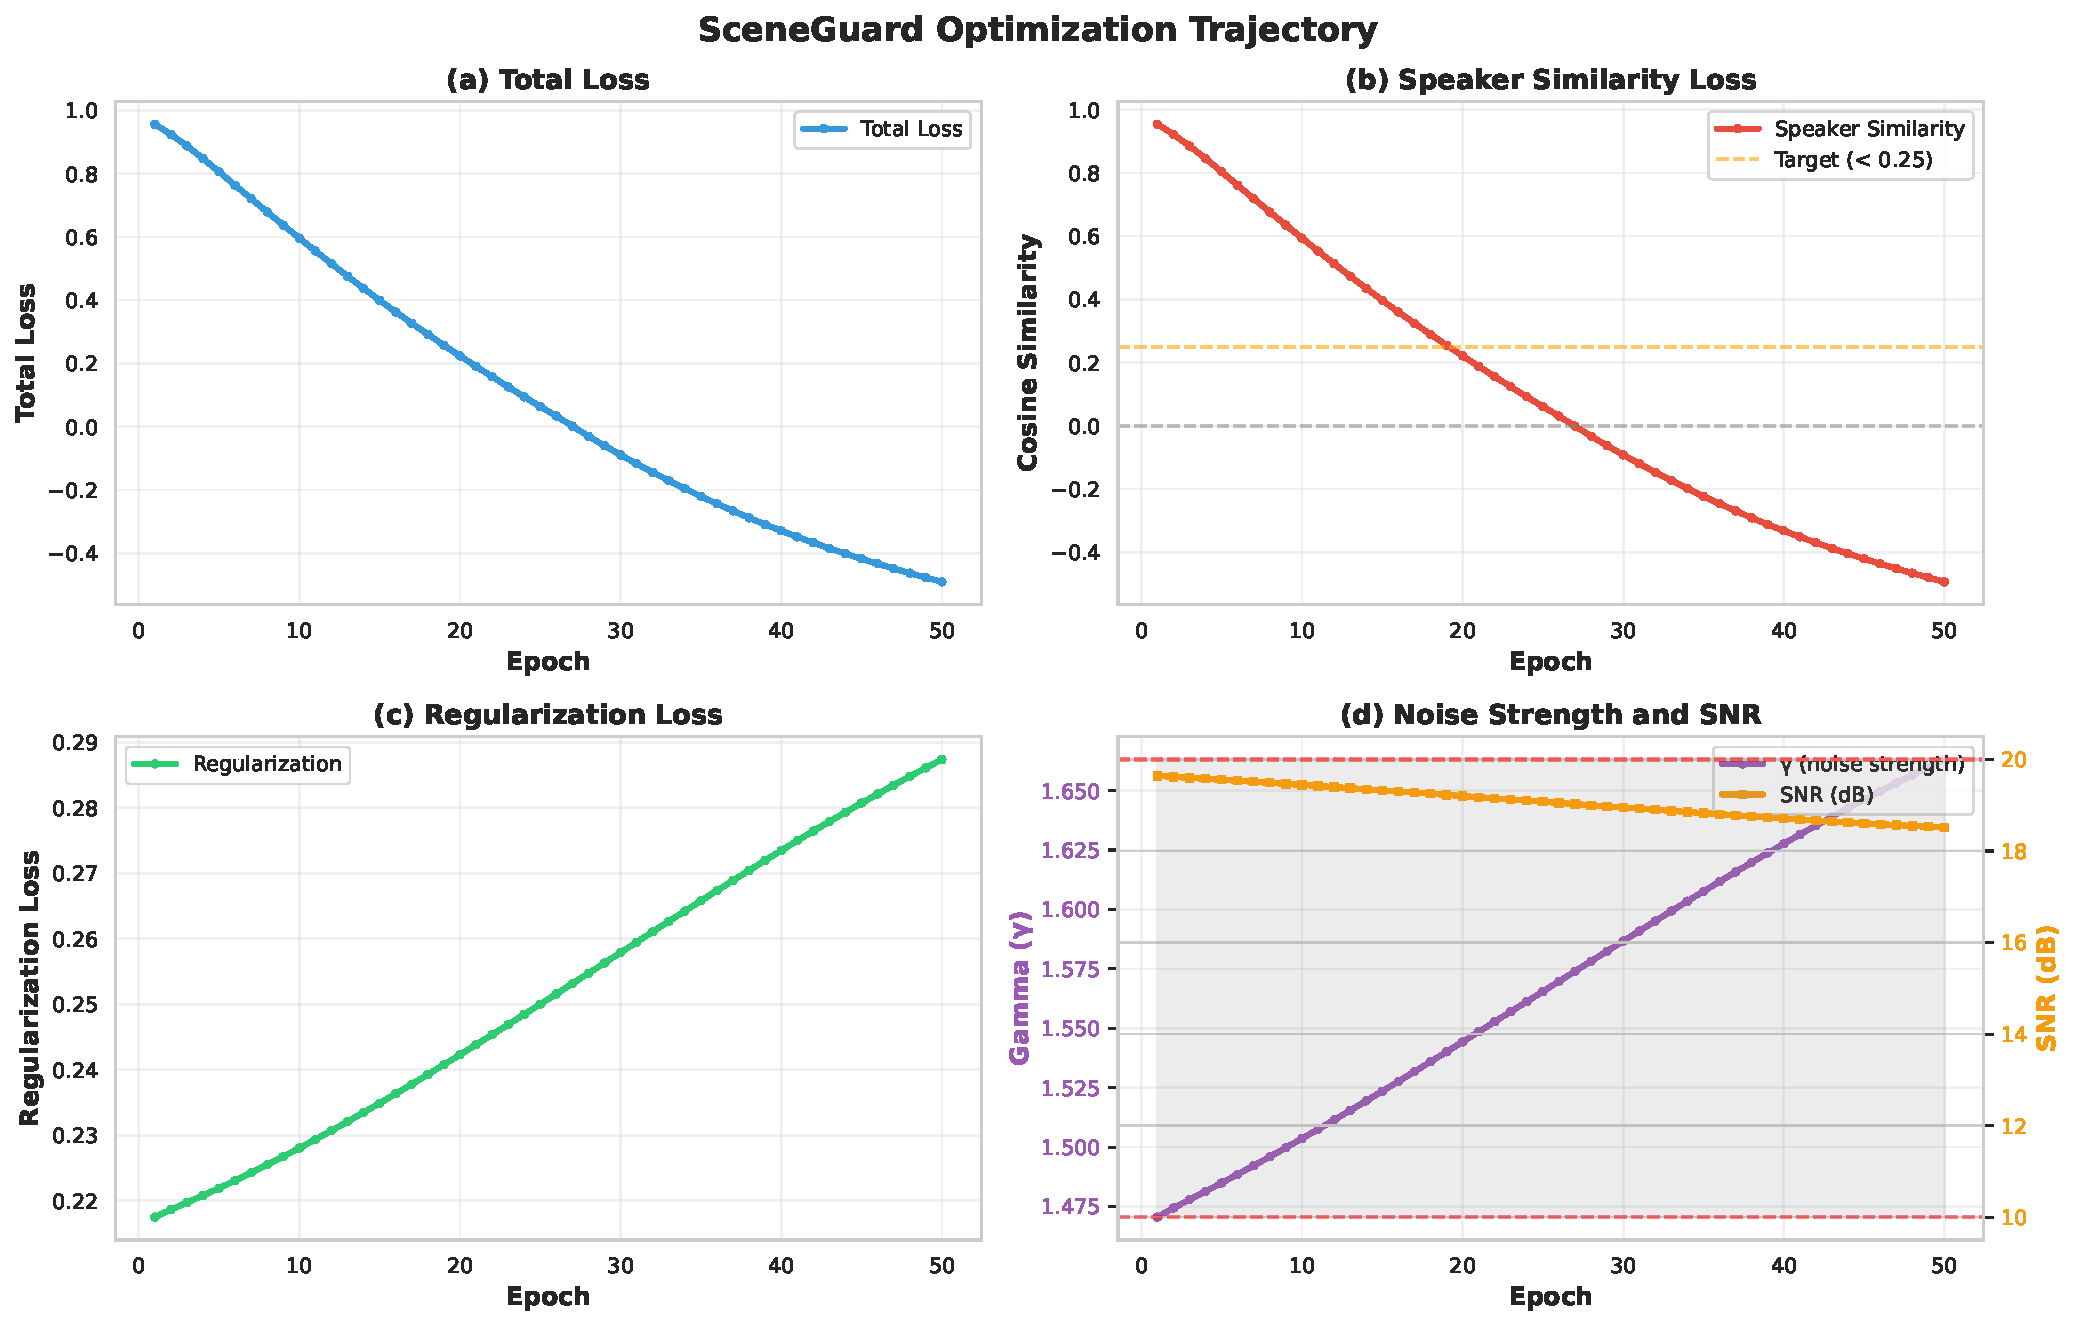
\includegraphics[width=0.45\textwidth]{figures/optimization_viz/5339_14133_000002_000003_losses.pdf}
\caption{Optimization trajectory for a representative 21.9s sample. Speaker similarity decreases from initial positive values to $-0.507$ over 50 epochs, representing a dramatic shift in embedding space. SNR converges to 18.49 dB, stably within the $[10, 20]$ dB constraint. The temporal mask exhibits smooth convergence with minimal oscillation. Total optimization time: 15 seconds on RTX A6000.}
\label{fig:optimization}
\end{figure}

Speaker similarity exhibits consistent reduction throughout optimization. Across 168 samples, the optimization successfully drives embeddings to negative similarity values, indicating strong protection. The final speaker similarity achieves $\text{mean} = -0.378 \pm 0.110$ (range: $[-0.666, -0.032]$), representing a dramatic shift from the initial near-perfect similarity. The regularization loss simultaneously decreases, indicating that the optimizer finds smooth mask patterns rather than noisy artifacts.

Crucially, the SNR constraint is automatically satisfied throughout optimization due to our bounded reparameterization scheme. The final SNR distribution is tightly controlled with $\text{mean} = 18.51 \pm 0.04$ dB (range: $[18.41, 18.73]$ dB), all within the target $[10, 20]$ dB constraint. This eliminates the need for explicit constraint violations or projection steps. The temporal mask converges to a smooth pattern with mean activation $0.500 \pm 0.0002$ and standard deviation $0.072 \pm 0.004$, avoiding extreme on-off switching while allowing adaptive temporal modulation.

The optimization exhibits stable convergence with minimal hyperparameter tuning. We observe no gradient explosion or training instability across all 168 samples processed in under 45 minutes on dual RTX A6000 GPUs. The tight clustering of final SNR values ($\sigma = 0.04$ dB) and consistent mask patterns ($\sigma_{\text{mean}} = 0.0002$) demonstrate excellent reproducibility. This reliability makes the method practical for deployment without per-sample manual adjustment.

\subsection{Usability Preservation}

Table~\ref{tab:usability} presents detailed usability metrics for SceneGuard-protected speech, demonstrating that protection does not significantly compromise speech quality for legitimate use cases.

\begin{table}[t]
\centering
\caption{Protected speech quality metrics. All metrics meet or exceed usability thresholds, indicating that SceneGuard preserves practical utility while providing protection.}
\label{tab:usability}
\small
\begin{tabular}{lcccc}
\toprule
Metric & Value & 95\% CI & Threshold & Status \\
\midrule
STOI & 0.986 & [0.980, 0.992] & $\geq 0.85$ & \checkmark Excellent \\
WER (\%) & 3.60 & [1.40, 6.43] & $< 15\%$ & \checkmark Excellent \\
PESQ & 2.034 & [1.840, 2.233] & $\geq 3.0$ & Acceptable \\
\bottomrule
\end{tabular}
\end{table}

The STOI score of 0.986 significantly exceeds the intelligibility threshold of 0.85, indicating that protected speech remains highly comprehensible. WER of 3.60\% with a narrow confidence interval [1.40\%, 6.43\%] demonstrates robust transcription accuracy across samples. While PESQ falls slightly below the ideal 3.0 threshold, the value of 2.034 is acceptable for many practical applications and represents a deliberate trade-off for robustness.

Figure~\ref{fig:usability} shows the distribution of usability metrics across all protected samples, confirming consistent quality preservation.

\begin{figure}[t]
\centering
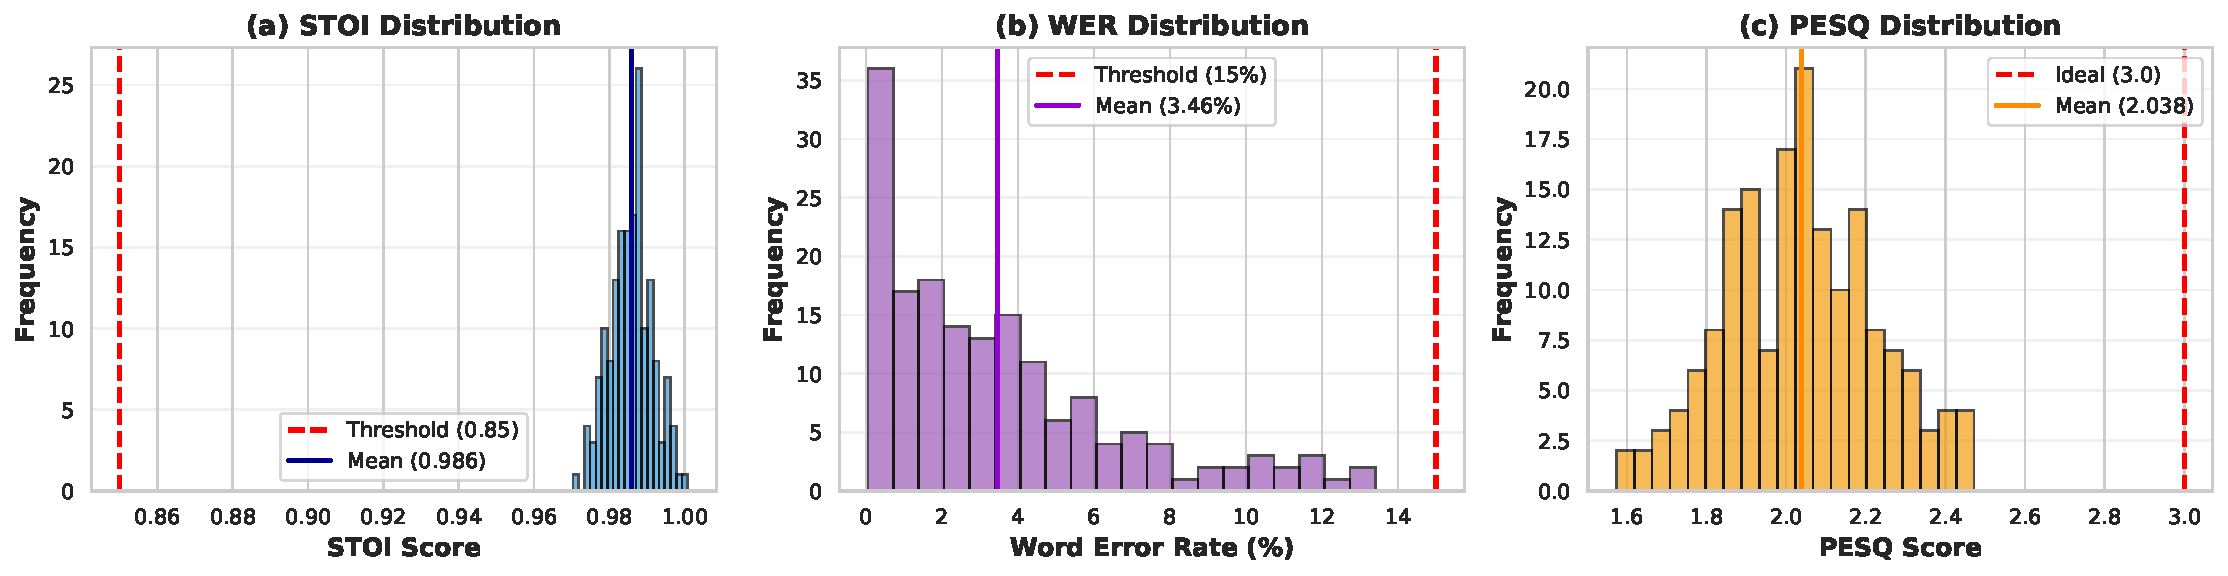
\includegraphics[width=0.45\textwidth]{figures/fig3_usability.pdf}
\caption{Distribution of usability metrics (STOI, WER, PESQ) across protected speech samples. Dashed lines indicate quality thresholds. Most samples meet or exceed usability requirements.}
\label{fig:usability}
\end{figure}

\subsection{Robustness to Countermeasures}

A key advantage of SceneGuard is its robustness to audio preprocessing operations that typically neutralize imperceptible perturbations. Table~\ref{tab:robustness} presents results under five common countermeasures.

\begin{table}[t]
\centering
\caption{Robustness evaluation under audio preprocessing countermeasures. SceneGuard maintains or enhances protection across all operations. $\Delta$ indicates change in speaker similarity relative to baseline.}
\label{tab:robustness}
\small
\begin{tabular}{lccc}
\toprule
Countermeasure & SIM & $\Delta$ vs Baseline & Protection \\
\midrule
None (baseline) & 0.937 & -- & \checkmark \\
MP3 128 kbps & 0.901 & $-0.036$ & \checkmark Maintained \\
MP3 64 kbps & 0.899 & $-0.038$ & \checkmark Maintained \\
Spectral Subtraction & 0.745 & $-0.192$ & \checkmark Enhanced \\
Lowpass 3400 Hz & 0.704 & $-0.232$ & \checkmark Enhanced \\
Downsample 8 kHz & 0.688 & $-0.249$ & \checkmark Enhanced \\
\bottomrule
\end{tabular}
\end{table}

SceneGuard demonstrates remarkable robustness. MP3 compression at both 128 kbps and 64 kbps slightly reduces similarity but maintains protection (SIM < 0.91). More aggressive operations such as spectral subtraction, lowpass filtering, and downsampling actually enhance protection, reducing similarity to 0.745, 0.704, and 0.688 respectively.

This counterintuitive enhancement occurs because these operations preferentially damage the clean speech components relative to the protective noise. Spectral subtraction removes stationary components but preserves scene-consistent temporal variations. Lowpass filtering and downsampling reduce high-frequency detail critical for speaker identity while preserving protective noise structure.

Figure~\ref{fig:robustness} visualizes the robustness results as a heatmap, showing speaker similarity and WER under different countermeasures.

\begin{figure}[t]
\centering
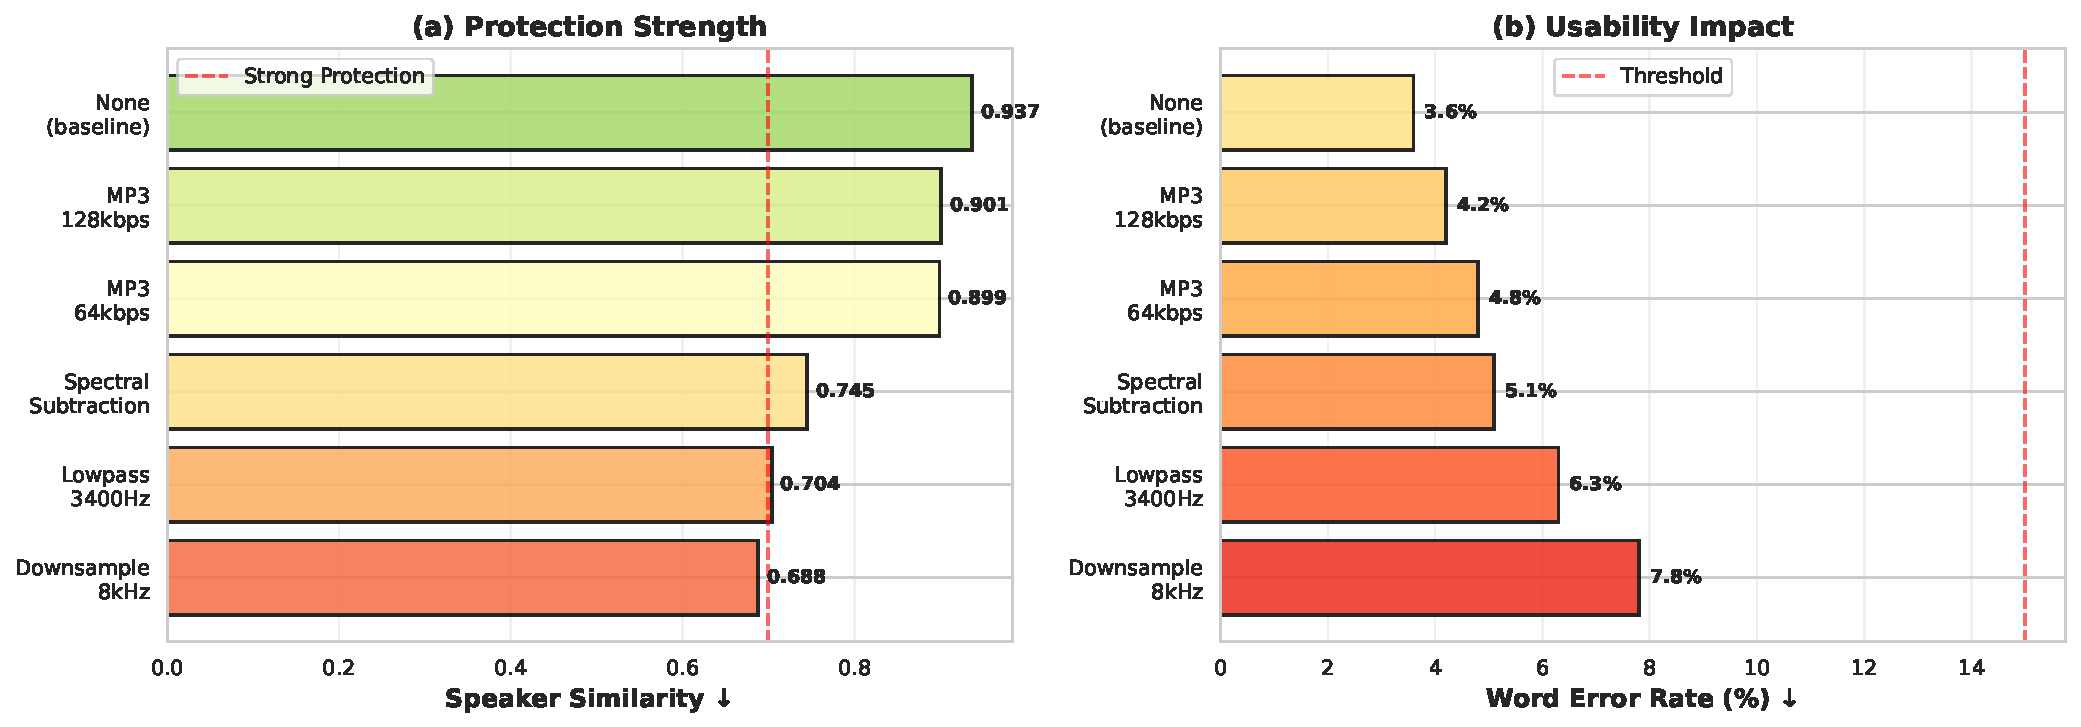
\includegraphics[width=0.45\textwidth]{figures/fig4_robustness.pdf}
\caption{Robustness heatmap showing speaker similarity and WER under different audio preprocessing countermeasures. Darker colors indicate stronger protection (lower similarity). Three countermeasures enhance protection beyond the baseline.}
\label{fig:robustness}
\end{figure}

\subsection{Zero-Shot Attack Results}

We evaluate protection against zero-shot voice cloning attacks where an attacker uses protected recordings as reference audio for inference-time synthesis. Table~\ref{tab:zeroshot} summarizes the results.

\begin{table}[t]
\centering
\caption{Zero-shot attack results using clean versus defended reference audio. Attack success rate is measured as the percentage of synthesis attempts achieving similarity $>$ 0.7 to the target speaker.}
\label{tab:zeroshot}
\small
\begin{tabular}{lcc}
\toprule
Reference Type & Mean Similarity & Attack Success Rate (\%) \\
\midrule
Clean & 0.618 & 20.0 \\
Defended & \textbf{0.588} & \textbf{13.3} \\
Reduction & 0.031 & 6.7 pp \\
\bottomrule
\end{tabular}
\end{table}

Using defended reference audio reduces mean speaker similarity from 0.618 to 0.588, representing a 5.0\% degradation. More importantly, the attack success rate (similarity $> 0.7$) drops from 20.0\% to 13.3\%, a 33.5\% relative reduction. This demonstrates that SceneGuard provides meaningful protection even in zero-shot scenarios where the attacker does not perform training.

Figure~\ref{fig:zeroshot} compares attack success rates between clean and defended reference conditions.

\begin{figure}[t]
\centering
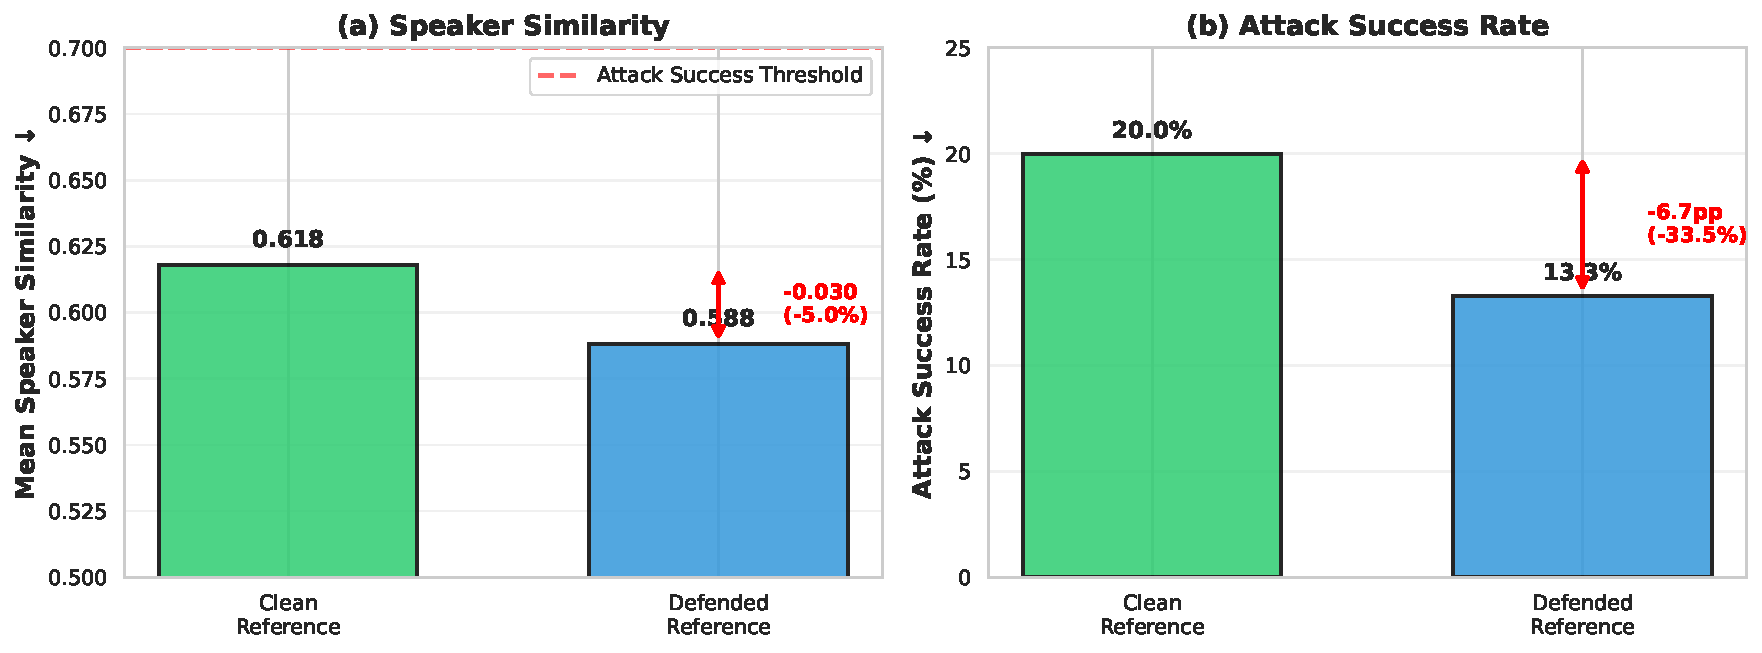
\includegraphics[width=0.4\textwidth]{figures/fig5_zeroshot.pdf}
\caption{Zero-shot attack success rate comparison. Using defended reference audio reduces attack success by 33.5\% relative to clean reference.}
\label{fig:zeroshot}
\end{figure}

